%\subsection{Event Slicing and Cosmic Removal in Pandora}

The work presented in this note relies on the Pandora approach for event reconstruction~\cite{bib:pandoraub}. The scope of Pandora is to do the low-level pattern-recognition step of the reconstruction, i.e. group hits into clusters, clusters into particles and particles into hierarchies. This section describes how Pandora's pattern-recognition output is combined with scintillation light information to isolate possible candidate neutrino interactions in MicroBooNE events, a process illustrates in the three images of figure~\ref{fig:sliceid}. 

\begin{figure}[ht] 
\begin{center}
    \begin{subfigure}[b]{0.7\textwidth}
    \centering
    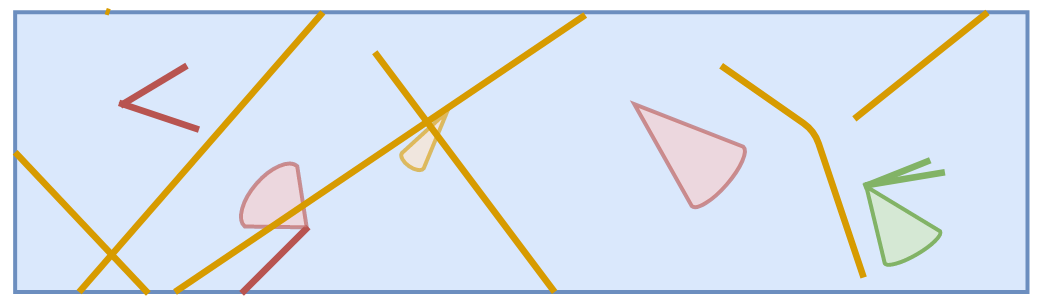
\includegraphics[width=1.00\textwidth]{NuId-Ch2/Images/slice00.png}
    \caption{\label{fig:slcieid:00} Typical event with multiple interactions isolated by Pandora in \emph{slices}.}
    \end{subfigure}
    \begin{subfigure}[b]{0.7\textwidth}
    \centering
    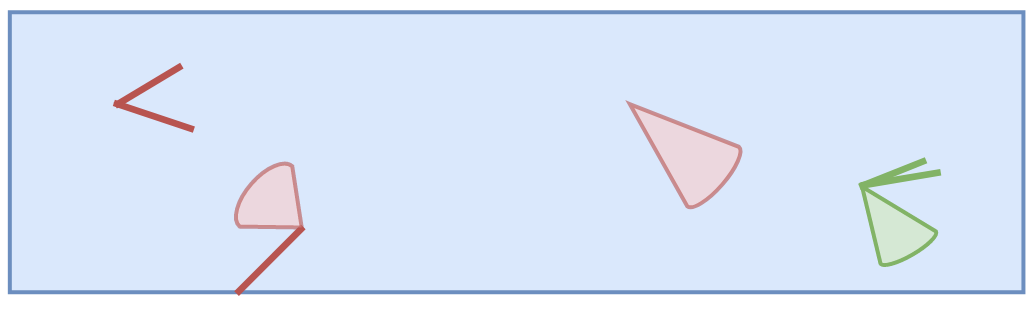
\includegraphics[width=1.00\textwidth]{NuId-Ch2/Images/slice01.png}
    \caption{\label{fig:slcieid:01} Event after the removal of \emph{obvious cosmics} tagged geometrically by Pandora.}
    \end{subfigure}
    \begin{subfigure}[b]{0.7\textwidth}
    \centering
    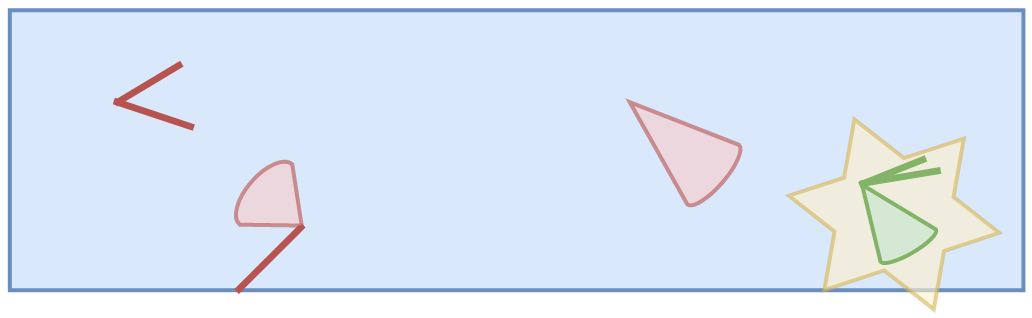
\includegraphics[width=1.00\textwidth]{NuId-Ch2/Images/slice02.png}
    \caption{\label{fig:slcieid:02} Implementation of the \texttt{SiceID} tool to isolate possible candidate $\nu$ interactions.}
    \end{subfigure}
\caption{\label{fig:sliceid} Succession of steps in cosmic removal performed using Pandora's topological pattern recognition combined with scintillation light information through the \texttt{SliceID} tool.}
\end{center}
\end{figure}

\subsection{Slicing, Clustering and Vertexing \textcolor{green}{Wouter ... P.R. Elena}}
The creation of a ``slice" is the first step of the Pandora processing. A slice is a collection of distinct reconstructed particles which belong to the same interaction (such as a cosmic muon and its Michel electron, or the muon and proton in a 1$\mu$1$p$ neutrino interaction). To produce slices, the Pandora Cosmic Pattern Recognition is first run over all hits, aiming to construct muon tracks and associated $\delta$-rays and Michel electrons under the cosmic hypothesis (fig.~\ref{fig:slcieid:00}). At this stage, obvious cosmic activity (through-going or out-of-time muons) is tagged using geometric information and discarded (fig.~\ref{fig:slcieid:01}). The remaining hit collection is used as input to the Pandora Consolidated Pattern Recognition which reconstruct slices under the neutrino hypothesis. Each slice is now reconstructed both under the cosmic hypothesis and the neutrino hypothesis. A typical event contains approximately 5 slices. 

%\subsubsection{Clustering and Vertex Finding \textcolor{green}{Wouter}} 
\par In order to reconstruct the interactions in 3D, Pandora needs to match the information from at least two different views and create a neutrino vertex. Pandora computes the 2D clustering on the hits in each slice and in each plane separately. Then, a number of 3D candidate vertices is created by finding positions that project down on to the ends of the available 2D clusters. All the possible vertex candidates are fed into the support vector machine (SVM) vertex selection, and the candidate with the highest SVM score is chosen. This 3D vertex is used to split any existing clusters that straddle the vertex. Then, the cluster matching algorithms are run, where the clusters are compared between views and modified to improve the matching.

\subsection{SliceID : Cosmic Removal through topology and scintillation-light \textcolor{green}{Wouter... P.R. Elena}}
\label{sec:sliceID:SliceID}
\par After the Pandora pattern-recognition algorithm suite has isolated individual interactions into reconstructed \emph{slices} and removed the obvious cosmics, the remaining task is to identify which (if any) slice is associated to a neutrino interaction. Scintillation light information is used to reject slices incompatible with light recorded in-time with the beam. Additionally, topological cuts aimed at rejecting stopping-muon events which enter the TPC are used. The \texttt{SliceID} is at the core of all neutrino selections performed in this analysis; this first, common step is responsible for the majority of cosmic-rejection.
\\
\par We leverage three handles to distinguish between neutrino and cosmic-ray slices:
\begin{enumerate}
    \item simple optical pre-selection cuts, which remove slices totally inconsistent with the beam flash;
    \item a topological score, which assesses to what extent the slice look like a neutrino interaction in the TPC;
    \item a flash-matching score, which assesses how well the flash-hypothesis for the slice matches the beam flash.
\end{enumerate}

\begin{comment}
To select the neutrino slice, or reject the event at this stage, the following procedure is followed:
\begin{itemize}
    \item Insist that there is a beam-triggered flash in the beam window.
    \item Only consider slices that pass the optical pre-selection cuts.
    \item If the slice with the largest topological score in the event remains, then select it as the neutrino.
    \item If not, then choose the remaining slice with the largest flash-matching score.
\end{itemize}
Further details on the \texttt{SliceID} tool are available in DocDB 23854 and 22519. Additional documentation for this tool is in preparation.
\end{comment}

To select the neutrino slice, we first require a beam-triggered flash in the beam window. 
Then, we apply the optical pre-selection cuts: if no slice passes optical pre-selection, the event is rejected. 
If the slice with the largest topological score passes the optical pre-selection, the slice forms the neutrino candidate; otherwise, the slice with the largest flash-matching score forms the neutrino candidate.
The performance of the \texttt{SliceID} for electron neutrino simulated events is given in~\cref{fig:sliceid}.

Further details on the \texttt{SliceID} tool are available in DocDB 23854 and 22519. Additional documentation for this tool is in preparation.



\begin{figure}[H]
    \centering
    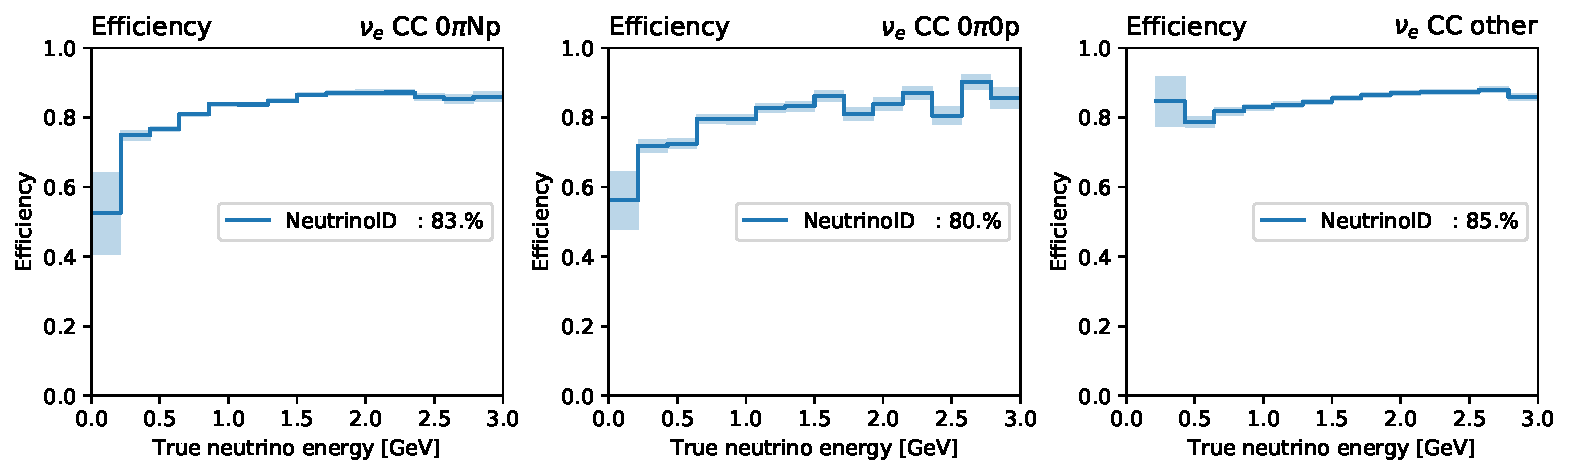
\includegraphics[width=\textwidth]{NuId-Ch2/Images/efficiency_cat_0.pdf}
    \caption{The performance of the \texttt{SliceID} as a function of the true neutrino energy for the topologies considered in the $\nu_e$ selection: the \npsel (left), the  \zpsel (middle) and inclusive (right) channels.}
    \label{fig:sliceid}
\end{figure}



\subsection{CRT Veto and Distance Tagger \textcolor{green}{Elena}}
\label{sec:sliceID:CRT}
Contrary to  $\nu_\mu$ interactions and cosmic rays, the charged particles associated to $\nu_e$ interactions are unlikely to deposit energy in the Cosmic Ray Tagger (CRT). Building upon this discriminating factor, the CRT Veto and CRT Distance Tagger are preselection tools which leverage the additional CRT information available for Run 3+ data.
When used, these CRT tools are applied at the pre-selection stage in the following order: CRT Veto, \texttt{SliceID}, CRT Distance Tagger. The CRT tools are especially impactful for the 1e0p channel, where discrimination handles based on the proton PID are obviously missing. \\


\emph{CRT Veto.} %On average, only one in six events passing the MicroBooNE common optical filter is associated to beam-induced activity. The remaining events are triggered by activity that originates outside the TPC: either external beam induced activity or cosmic rays. %Given the $\mathcal{O}(10)$ cosmic ray muons in each drift window, this equates to a starting signal-to-background of $\sim 1 : 60$.
%The CRT Veto looks at CRT activity in time with the beam window. 
The CRT veto looks for a time coincidence between the scintillation light recorded in time with the 1.6 $\mu$s beam-spill (beam-flash) and a CRT hit: if a CRT hit occurs within a 1 $\mu s$ of the beam flash, the event is rejected. For this coincidence, only CRT hits with PE $>$ 100 pe are considered; we do not apply a constraint on the position of the flash nor on the position of the CRT hit. 
The rejection power and efficiency of the CRT veto are calculated using the BNB external and the $\nu_e$ overlay samples, respectively. The BNB external passing rate is $\sim$59\%,  and the $\nu_e$ efficiency greater than $\sim$94\% for all electron neutrino energies, raising at low energies. \\


\emph{CRT Distance Tagger.} 
The CRT Distance Tagger tool builds upon the standard pandora neutrino vertex reconstruction and the CRT tagging of TPC tracks. A TPC track is tagged with a CRT hit association if the track projection onto a CRT panel and a CRT hit are close in space. 
To perform this association, the track projection to the CRT is calculated under the hypothesis that the associated particle crossed the TPC at the time registered by the CRT hit under consideration; more details on the CRT hit to TPC track match are available in \cite{bib:CRTPresel_Technote}.  The CRT Distance Tagger checks the minimum distance between the reconstructed neutrino vertex and each track tagged with a CRT hit. If the minimum distance is less than 14 cm, the event is rejected. An example event tagged by this cut is shown in Figure~\ref{fig:crtdist00}.  For the CRT Distance Tagger, the BNB external passing rate is $\sim$81\%,  and the $\nu_e$ efficiency greater than $\sim$96\% for all electron neutrino energies, raising at low energies. \\
 
\begin{figure}[h!]
\centering
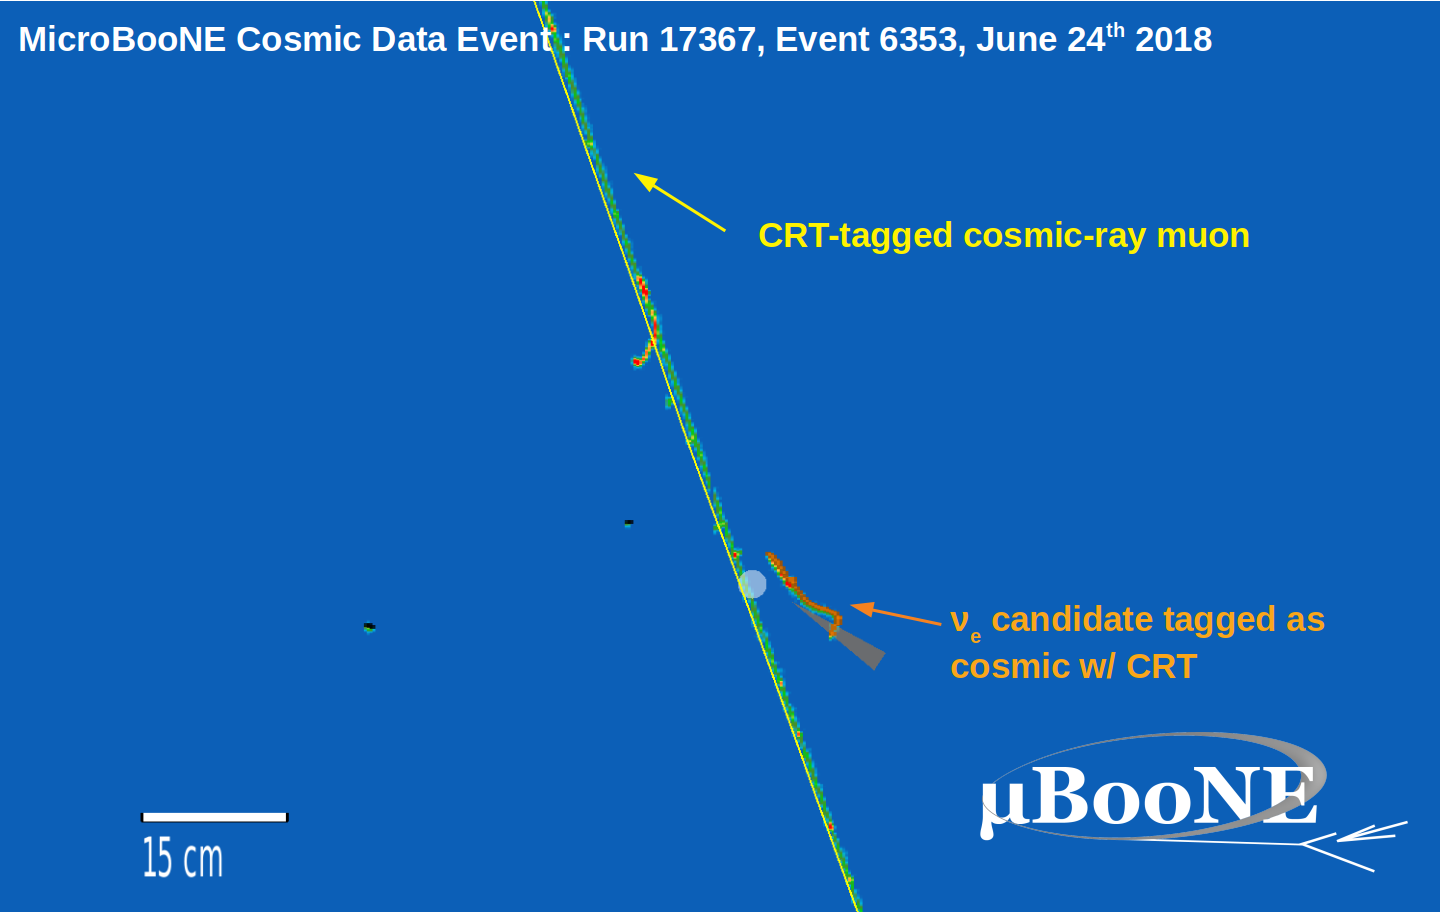
\includegraphics[width=0.4\textwidth]{NuId-Ch2/Images/crttagger_01.png}
\caption{Example $\nu_e$ candidate tagged as cosmic thanks to the CRT distance tagger. From the event one can see that the reconstructed EM shower is associated to EM activity associated to the incoming muon.}
\label{fig:crtdist00}
\end{figure}

An overview of the impact of the CRT on cosmic rejection can be seen in Figure~\ref{fig:crt} where the beam-time distribution for the $8E18$ POT Run 3 open dataset is shown after \texttt{SliceID} (left), and after \texttt{SliceID} and CRT cosmic-tagging tools (both CRT veto and distance tagger) have been applied (right), with EXT backgrounds dropping by more than a factor of 3.
Further details and a preliminary study of the CRT  impact on an electron neutrino preselection can be found in \cite{bib:CRTPresel_Technote}. 

\begin{figure}[ht] 
\begin{center}
    \begin{subfigure}[b]{0.4\textwidth}
    \centering
    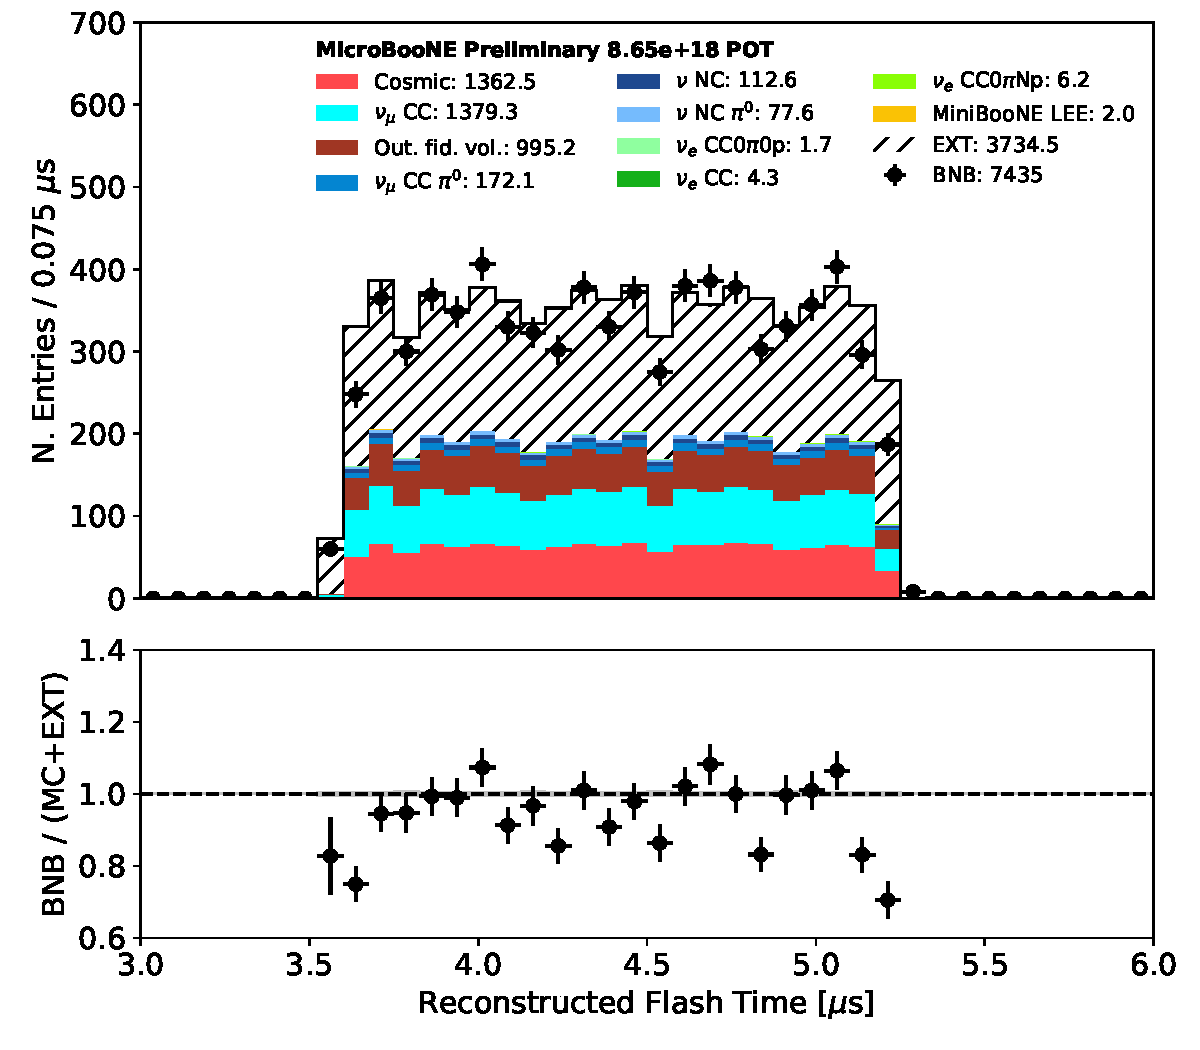
\includegraphics[width=1.00\textwidth]{NuId-Ch2/Images/flash_time_01152020.pdf}
    \caption{\label{fig:crt:pre} no CRT tools.}
    \end{subfigure}
    \begin{subfigure}[b]{0.4\textwidth}
    \centering
    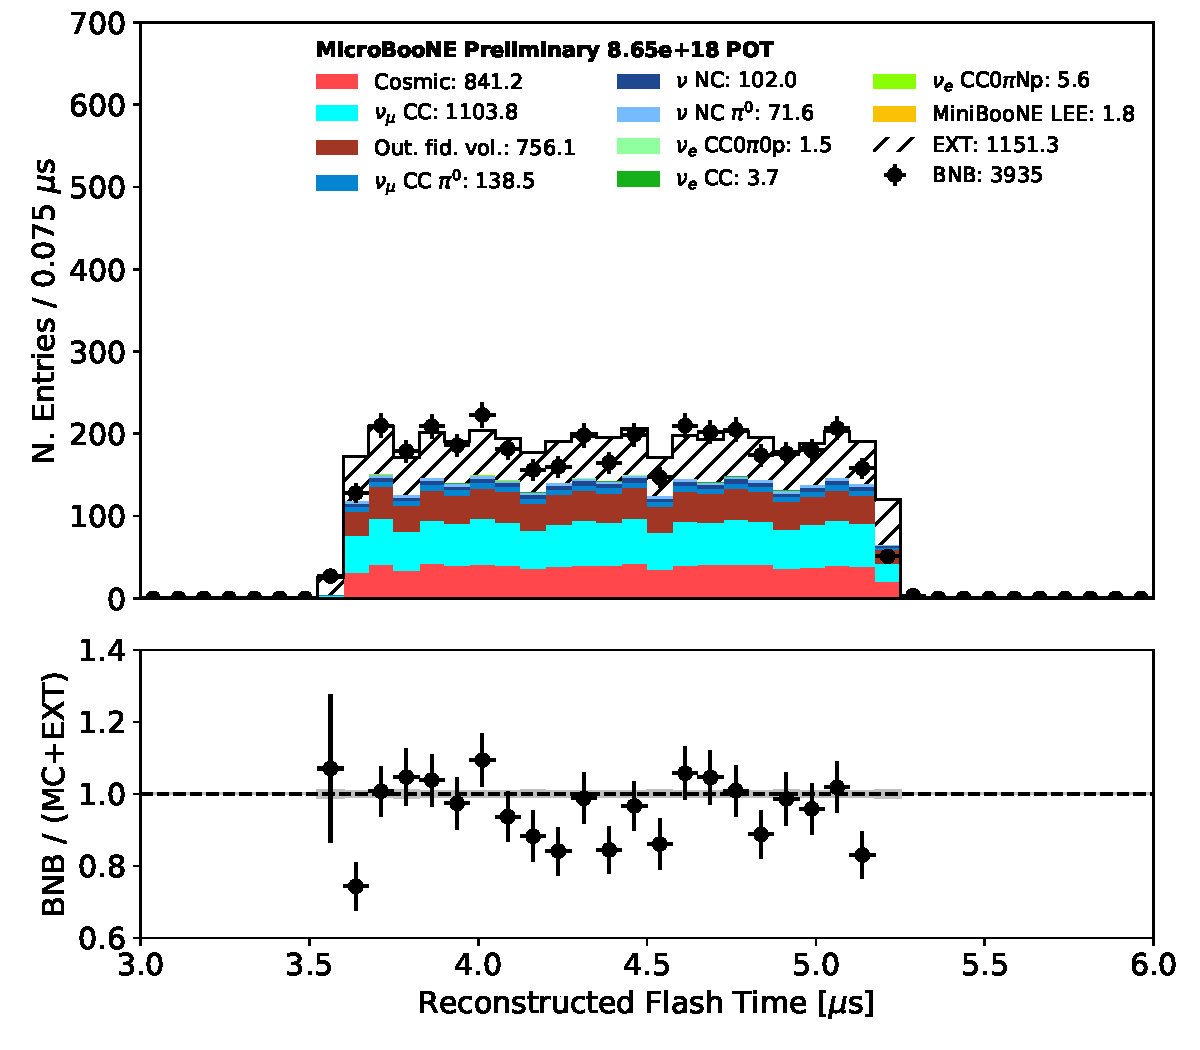
\includegraphics[width=1.00\textwidth]{NuId-Ch2/Images/flash_time_01152020_CRT.pdf}
    \caption{\label{fig:crt:post} with CRT tools.}
    \end{subfigure}
\caption{\label{fig:crt} Beam timing distribution before (left) and after (right) CRT tools have been applied. The EXT contribution is reduced by over a factor of three.}
\end{center}
\end{figure}